%&<latex>
\documentclass[letterpaper,12pt]{article}

%%%%%%%%%%%%%%%%%%%%%%%%%%%%%%%%%%%%%%%%%%%%%%%%%%%%%%%%%%%%
%% preamble %%%%%%%%%%%%%%%%%%%%%%%%%%%%%%%%%%%%%%%%%%%%%%%%
\pdfpagewidth = 8.5in
\pdfpageheight = 11.0in
\usepackage[left=1in,right=1in,top=1in,bottom=1in]{geometry}

\pagestyle{plain}
\pagenumbering{arabic}
\usepackage{setspace}
\usepackage[fleqn]{amsmath}
\usepackage{amssymb}
\usepackage{graphicx}
\usepackage{url}
\usepackage{verbatim}
\usepackage{appendix}
\usepackage{indentfirst}
\usepackage{booktabs}
\usepackage{multirow}
\usepackage{ragged2e}
\usepackage{upgreek}
\usepackage[T1]{fontenc}
\usepackage[titles]{tocloft}
\usepackage{xspace}
\usepackage[usenames]{color}
\usepackage{ifthen}
\usepackage{cancel}
\usepackage{array}
\usepackage{tabulary}
\usepackage{authblk}
\usepackage{tikz}
\usepackage{pdflscape}

%% Set up color palettes %%%%%%%%%%%%%%%%%%%%%%%%%%%%%%%%%%%%%%%%%%%%
% Color palette GreenOrange_6 from
% https://jiffyclub.github.io/palettable/tableau/
\definecolor{pgreen}     {RGB}{50,162,81}
\definecolor{porange}    {RGB}{255,127,15}
\definecolor{pblue}      {RGB}{60,183,204}
\definecolor{pyellow}    {RGB}{255,217,74}
\definecolor{pteal}      {RGB}{57,115,124}
\definecolor{pauburn}    {RGB}{184,90,13}
%%%%%%%%%%%%%%%%%%%%%%%%%%%%%%%%%%%%%%%%%%%%%%%%%%%%%%%%%%%%%%%%%%%%%

\usepackage{hyperref}
\hypersetup{pdfborder={0 0 0},
            colorlinks=true,
            urlcolor=porange,
            linkcolor=pauburn,
            citecolor=pteal}

\usepackage[capitalize]{cleveref}
\newcommand{\crefrangeconjunction}{--}

% Set up line numbering; using lineno to number lines of paragraphs with
% equations sanely
\usepackage[right, mathlines]{lineno}
\setlength\linenumbersep{1cm}
\def\linenumberfont{\normalfont\scriptsize\sffamily}

% Set up caption formatting
\usepackage{subcaption}
\usepackage[format=plain, labelsep=period, singlelinecheck=true, skip=2pt, font=sf]{caption}
\DeclareCaptionLabelFormat{noSpace}{{#1}{#2}}
\DeclareCaptionListFormat{figList}{Figure {#2}.}
\DeclareCaptionListFormat{sFigList}{Figure S{#2}.}

% Define tightly formated list environments via enumitem
\usepackage{enumitem}
\newenvironment{tightItemize}{%
\begin{itemize}[noitemsep, topsep=0pt, parsep=0pt, partopsep=0pt]}
{\end{itemize}}

\newenvironment{veryTightItemize}{%
\begin{itemize}[noitemsep, topsep=0pt, parsep=0pt, partopsep=0pt, leftmargin=*]}
{\end{itemize}}

\newenvironment{tightEnumerate}{%
\begin{enumerate}[noitemsep, topsep=0pt, parsep=0pt, partopsep=0pt]}
{\end{enumerate}}

\newenvironment{veryTightEnumerate}{%
\begin{enumerate}[noitemsep, topsep=0pt, parsep=0pt, partopsep=0pt, leftmargin=*]}
{\end{enumerate}}

\newcommand{\citationNeeded}{\textcolor{magenta}{\textbf{[CITATION NEEDED!]}}\xspace}
\newcommand{\tableNeeded}{\textcolor{magenta}{\textbf{[TABLE NEEDED!]}}\xspace}
\newcommand{\figureNeeded}{\textcolor{magenta}{\textbf{[FIGURE NEEDED!]}}\xspace}
\newcommand{\highLight}[1]{\textcolor{magenta}{\MakeUppercase{#1}}}

\newcommand{\editorialNote}[1]{\textcolor{red}{[\textit{#1}]}}
\newcommand{\ignore}[1]{}
\newcommand{\addTail}[1]{\textit{#1}.---}
\newcommand{\super}[1]{\ensuremath{^{\textrm{#1}}}}
\newcommand{\sub}[1]{\ensuremath{_{\textrm{#1}}}}
\newcommand{\dC}{\ensuremath{^\circ{\textrm{C}}}}
\newcommand{\tb}{\hspace{2em}}
\newcommand{\tn}{\tabularnewline}
\newcommand{\spp}[1]{\textit{#1}}

\providecommand{\e}[1]{\ensuremath{\times 10^{#1}}}

\newcommand{\change}[2]{{\color{red} #2}\xspace}
\newcommand{\thought}[1]{\textcolor{purple}{THOUGHT: #1}}

\newcommand{\widthFigure}[5]{\begin{figure}[htbp]
\begin{center}
    \includegraphics[width=#1\textwidth]{#2}
    \captionsetup{#3}
    \caption{#4}
    \label{#5}
    \end{center}
    \end{figure}}

\newcommand{\heightFigure}[5]{\begin{figure}[htbp]
\begin{center}
    \includegraphics[height=#1]{#2}
    \captionsetup{#3}
    \caption{#4}
    \label{#5}
    \end{center}
    \end{figure}}

\newcommand{\smartFigure}[4]{%
    \begin{figure}[htbp]
        \begin{center}
            % \includegraphics[width=\textwidth,height=0.95\textheight,keepaspectratio]{#1}
            \includegraphics[width=\textwidth,height=0.89\textheight,keepaspectratio]{#1}
            \captionsetup{#2}
            \caption{#3}
            \label{#4}
        \end{center}
    \end{figure}
}

\newcommand{\mFigure}[3]{\smartFigure{#1}{listformat=figList}{#2}{#3}\clearpage}
\newcommand{\embedHeightFigure}[4]{\heightFigure{#1}{#2}{listformat=figList}{#3}{#4}}
\newcommand{\embedWidthFigure}[4]{\widthFigure{#1}{#2}{listformat=figList}{#3}{#4}}
\newcommand{\siFigure}[3]{\smartFigure{#1}{name=Figure S, labelformat=noSpace, listformat=sFigList}{#2}{#3}\clearpage}

\newcommand{\weusedggplot}{Figure generated with ggplot2 Version 2.2.1
    \citep{ggplot2}.}
\newcommand{\weusedggridges}{Figure generated with ggridges Version 0.4.1
    \citep{ggridges041} and ggplot2 Version 2.2.1 \citep{ggplot2}.}

\newcommand{\given}{\ensuremath{\,|\,}\xspace}
\newcommand{\pr}{\ensuremath{p}}

\newcommand{\data}{\ensuremath{D}\xspace}
\newcommand{\model}[1][]{\ensuremath{M_{#1}}\xspace}
\newcommand{\parameters}[1][]{\ensuremath{\Theta_{#1}}\xspace}
\newcommand{\diff}[1]{\ensuremath{\mathrm{d}#1}}

\newcommand{\distgamma}{\ensuremath{\textrm{Gamma}}\xspace}
\newcommand{\distexponential}{\ensuremath{\textrm{Exponential}}\xspace}
\newcommand{\dgamma}[2]{\ensuremath{\distgamma(\textrm{shape} = #1, \textrm{mean} = #2)}}
\newcommand{\dexponential}[1]{\ensuremath{\distexponential(\textrm{mean} = #1)}}

\newcommand{\ncomparisons}{\ensuremath{n\xspace}}
\newcommand{\nevents}[1][]{\ensuremath{k_{#1}\xspace}}
\newcommand{\nloci}[1][]{\ensuremath{m_{#1}\xspace}}

\newcommand{\observedallelecount}[1][]{\ensuremath{n_{#1}}\xspace}
\newcommand{\observedredallelecount}[1][]{\ensuremath{r_{#1}}\xspace}

\newcommand{\nodeallelecount}[2]{\ensuremath{n_{#1}^{#2}}}
\newcommand{\noderedallelecount}[2]{\ensuremath{r_{#1}^{#2}}}

\newcommand{\allelecount}[1][]{\ensuremath{\nodeallelecount{#1}{}}\xspace}
\newcommand{\redallelecount}[1][]{\ensuremath{\noderedallelecount{#1}{}}\xspace}

\newcommand{\leafallelecounts}[1][]{\ensuremath{\mathbf{n}_{#1}}\xspace}
\newcommand{\leafredallelecounts}[1][]{\ensuremath{\mathbf{r}_{#1}}\xspace}
\newcommand{\maxleafallelecounts}{\ensuremath{\textrm{max}(\mathbf{n})}\xspace}

\newcommand{\comparisondata}[1][]{\ensuremath{D_{#1}}\xspace}
\newcommand{\alldata}[1][]{\ensuremath{\mathbf{D}}\xspace}

\newcommand{\branchindex}{\ensuremath{x}\xspace}
\newcommand{\allelecountbottom}[1][\branchindex]{\nodeallelecount{#1}{B}}
\newcommand{\allelecounttop}[1][\branchindex]{\nodeallelecount{#1}{T}}
\newcommand{\redallelecountbottom}[1][\branchindex]{\noderedallelecount{#1}{B}}
\newcommand{\redallelecounttop}[1][\branchindex]{\noderedallelecount{#1}{T}}

\newcommand{\msbayes}{\upshape\texttt{msBayes}\xspace}
\newcommand{\dppmsbayes}{\upshape\texttt{dpp-msbayes}\xspace}
\newcommand{\cpp}{\upshape\texttt{C++}\xspace}
\newcommand{\ecoevolity}{\upshape\texttt{ecoevolity}\xspace}
\newcommand{\simcoevolity}{\upshape\texttt{simcoevolity}\xspace}
\newcommand{\sumcoevolity}{\upshape\texttt{sumcoevolity}\xspace}
\newcommand{\pycoevolity}{\upshape\texttt{pycoevolity}\xspace}

\newcommand{\rgmurate}{\ensuremath{u}\xspace}
\newcommand{\grmurate}{\ensuremath{v}\xspace}
\newcommand{\murate}[1][]{\ensuremath{\mu_{#1}}\xspace}
\newcommand{\murates}[1][]{\ensuremath{\boldsymbol{\mu}_{#1}}\xspace}
\newcommand{\gfreq}[1][]{\ensuremath{\pi_{#1}}\xspace}
\newcommand{\gfreqs}[1][]{\ensuremath{\boldsymbol{\pi}_{#1}}\xspace}

\newcommand{\comparisondivtime}[1][]{\ensuremath{t_{#1}}\xspace}
\newcommand{\comparisondivtimes}[1][]{\ensuremath{\mathbf{t}_{#1}}\xspace}
\newcommand{\divtime}[1][]{\ensuremath{\tau_{#1}}\xspace}
\newcommand{\divtimes}[1][]{\ensuremath{\boldsymbol{\tau}_{#1}}\xspace}
\newcommand{\divtimemodel}[1][]{\ensuremath{T_{#1}}\xspace}
\newcommand{\divtimesets}{\ensuremath{\mathcal{T}}\xspace}
\newcommand{\genetree}[1][]{\ensuremath{g_{#1}}\xspace}
\newcommand{\sptree}[1][]{\ensuremath{S_{#1}}\xspace}
\newcommand{\sptrees}[1][]{\ensuremath{\mathbf{S}_{#1}}\xspace}

\newcommand{\descendantpopindex}[1]{\ensuremath{D{#1}}}
\newcommand{\rootpopindex}[1][]{\ensuremath{R{#1}}\xspace}
\newcommand{\epopsize}[1][]{\ensuremath{N_{e}^{#1}}\xspace}
\newcommand{\comparisonpopsizes}[1][]{\ensuremath{\mathbb{N}_{e}{#1}}\xspace}
\newcommand{\collectionpopsizes}[1][]{\ensuremath{\mathbf{N_{e}}_{#1}}\xspace}
\newcommand{\rootrelativepopsize}{\ensuremath{R_{\epopsize[\rootpopindex]}}\xspace}

\newcommand{\dirp}{\ensuremath{\textrm{DP}}\xspace}
\newcommand{\concentration}{\ensuremath{\alpha}\xspace}
\newcommand{\basedistribution}{\ensuremath{H}\xspace}
\newcommand{\gshape}{\ensuremath{k}\xspace}
\newcommand{\gscale}{\ensuremath{\theta}\xspace}

\newcommand{\multiplier}{\ensuremath{m}\xspace}
\newcommand{\proposed}{\ensuremath{^{*}}\xspace}
\newcommand{\tuningparameter}{\ensuremath{\lambda}\xspace}
\newcommand{\uniformdeviate}{\ensuremath{u}\xspace}
\newcommand{\sizechange}{\ensuremath{\delta}\xspace}


\usepackage{media9}

% \newcommand{\ifembed}[2]{#1}
\newcommand{\ifembed}[2]{#2}
\newcommand{\ifdoublespacing}[2]{#1}
% \newcommand{\ifdoublespacing}[2]{#2}
\newcommand{\iflinenumbers}[2]{#1}
% \newcommand{\iflinenumbers}[2]{#2}
% \newcommand{\ifragged}[2]{#1}
\newcommand{\ifragged}[2]{#2}
% \newcommand{\ifblind}[2]{#1}
\newcommand{\ifblind}[2]{#2}

\usepackage[round]{natbib}

% \newcommand{\jroedit}[2]{\sout{#1}{\color{pauburn}{#2}}}
\newcommand{\jroedit}[2]{#2}
% \newcommand{\jroeditb}[2]{\sout{#1}{\color{pauburn}{#2}}}
\newcommand{\jroeditb}[2]{#2}
% \newcommand{\jroeditnote}[1]{[{\color{pauburn}{EDIT NOTE:}} \textbf{\color{pauburn}{#1}}]}
\newcommand{\jroeditnote}[1]{}
% \newcommand{\jroeditnoteb}[1]{[{\color{pauburn}{EDIT NOTE:}} \textbf{\color{pauburn}{#1}}]}
\newcommand{\jroeditnoteb}[1]{}
% \newcommand{\jroedithighlight}[1]{\color{pauburn}{#1}}
\newcommand{\jroedithighlight}[1]{#1}
\newcommand{\jrocomment}[1]{({\color{pgreen}{JRO's comment:}} \textbf{\color{pgreen}{#1}})}

\newcommand{\mstitle}{The comparative biogeography of \jroedit{}{Philippine} geckos
    challenges predictions from
    a paradigm of climate-driven vicariant diversification across an
    island archipelago}

\title{\mstitle}

\ifblind{\author{}}{
\author[1]{Jamie R.\ Oaks \thanks{Corresponding author: \href{mailto:joaks@auburn.edu}{\tt joaks@auburn.edu}}}
\author[2]{Cameron D.\ Siler}
\author[3]{Rafe M.\ Brown}
\affil[1]{Department of Biological Sciences \& Museum of Natural History,
    Auburn University, Auburn, Alabama 36849, USA}
\affil[2]{Sam Noble Oklahoma Museum of Natural History and Department of
    Biology, University of Oklahoma, Norman, Oklahoma 73072-7029}
\affil[3]{Biodiversity Institute and Department of Ecology and Evolutionary
    Biology, University of Kansas, Lawrence, Kansas 66045, USA}
}

\date{\today}
% \date{\parbox{\linewidth}{\centering%
%     \today\endgraf\bigskip
%     \textbf{Running head}: Comparative biogeography of Philippine geckos}}

\makeatletter
\let\msTitle\@title
\let\msAuthor\@author
\let\msDate\@date
\makeatother
%%%%%%%%%%%%%%%%%%%%%%%%%%%%%%%%%%%%%%%%%%%%%%%%%%%%%%%%%%%%
%%%%%%%%%%%%%%%%%%%%%%%%%%%%%%%%%%%%%%%%%%%%%%%%%%%%%%%%%%%%

\begin{document}

\ifragged{
\raggedright
}{}

\iflinenumbers{
\begin{linenumbers}
}{}

\textbf{Running head}: Comparative biogeography of Philippine geckos

\vspace{-1.3cm}
{\let\newpage\relax\maketitle}

\vspace{-1.8cm}
\section*{Author contributions}
\vspace{-4mm}
\ifblind{REDACTED}{%
J.R.O., C.D.S., and R.M.B.\ conceived the study.
R.M.B.\ and C.D.S.\ conducted fieldwork.
J.R.O.\ collected, assembled, and analyzed the sequence data.
J.R.O. led the writing of the manuscript, with contributions from C.D.S. and
R.M.B.}


\vspace{-7mm}
\section*{Acknowledgments}
\vspace{-4mm}
\ifblind{REDACTED}{
\jroedit{}{%
We thank the members of the Phyletica Lab (the phyleticians) for helpful
feedback on multiple drafts of this paper.
We also thank editors Mohamed Noor and David Weisrock and three anonymous
reviewers for constructive feedback that greatly improved this work.}
The computation\jroedit{}{al} work was made possible by
\jroedit{}{the}
Auburn University (AU) Hopper Cluster
supported by the AU Office of Information Technology
and
\jroedit{}{a grant of high-performance computing resources and technical
    support from the Alabama Supercomputer Authority.}
This work was possible thanks to funding provided to JRO from the National
Science Foundation (DBI 1308885 and DEB 1656004).
RMB's \jroedit{}{Philippines} research has been supported by NSF DEB 0073199, 0743491, 0640737,
1418895, and 1654388; and the University of Kansas Biodiversity Institute.
This paper is contribution number \highLight{XXXX} of the Auburn University
Museum of Natural History.
}


\vspace{-7mm}
\section*{Data Accessibility}
\vspace{-4mm}
All of the demultiplexed, raw sequence reads are available from the NCBI
Sequence Read Archive
(\ifblind{REDACTED}{Bioproject PRJNA486413, SRA Study SRP158258}).
A detailed history of all aspects of this project was recorded in a
version-controlled repository, which is publicly available at
\ifblind{REDACTED}{\url{https://github.com/phyletica/gekgo}},
and was archived on zenodo
(\url{https://dx.doi.org/10.5281/zenodo.2642461}).
Supplemental Tables 1 and 2 and the animation from Supplemental Figure 2 are
also available from the Dryad Digital Repository:
\url{https://doi.org/10.5061/dryad.n34d4m7}.


\newpage

\ifdoublespacing{
\doublespacing
}{}

\begin{center}
    {\Large \mstitle}
\end{center}

\begin{abstract}
    A primary goal of biogeography is to understand how large-scale environmental
processes, like climate change, affect diversification.
One often-invoked but seldom tested process is the \jroedit{so-called}{} ``species-pump''
model, in which repeated bouts of co-speciation \jroeditb{is}{are} driven by oscillating
climate-induced habitat connectivity cycles.
For example, over the past three million years, the landscape of the Philippine
Islands has repeatedly coalesced and fragmented due to sea-level changes
associated with \jroedit{the}{} glacial cycles.
This repeated climate-driven vicariance has been proposed as a model of
speciation across evolutionary lineages codistributed throughout the islands.
This model predicts speciation times that are temporally clustered around
the times when interglacial rises in sea level fragmented the islands.
% \jroedit{Given the significance and conceptual impact the model has shown, surprisingly
% few tests of this prediction have been provided.}{}
\jroedit{}{To test this prediction,}
\jroedit{We}{we} collected comparative genomic data from 16 pairs of insular gecko populations.
% \jroedit{to test the prediction of temporally clustered divergences.}{}
\jroedit{Specifically, we}{We} analyze these data in a full-likelihood, Bayesian model-choice
framework to test for shared divergence times among the pairs.
Our results provide support against the species-pump model prediction in favor
of an alternative interpretation, namely that each pair of gecko populations
diverged independently.
These results suggest the repeated bouts of climate-driven landscape
fragmentation has not been an important mechanism of speciation for
gekkonid lizards on the Philippine Islands.
% \jroedit{Interpretations of shared mechanisms of diversification historically have been
% pervasive in biogeography, often advanced on the basis of taxonomy-based
% depictions of species distributions.
% Our results call for possible re-evaluation of other, classic
% co-diversification studies in a variety of geographic systems.}{}


    \vspace{12pt}
    \noindent\textbf{KEY WORDS: biogeography, diversification, Philippines, phylogeography} 
\end{abstract}

\newpage

\section{Introduction}

Understanding how environmental changes affect diversification is an important
goal in evolutionary biology, biogeography, and global change biology.
Environmental processes that operate at or above the level of communities can
simultaneously cause speciation or extinction across multiple evolutionary
lineages, and thus have a pronounced effect on the diversity and distribution
of species.
% across an area.
Island archipelagos that harbor diverse communities of co-distributed lineages
and have a relatively well-understood geological history present powerful
systems for understanding such shared processes of diversification
\citep{Gillespie2007,Losos2009,Vences2009,Rafe2013AREES}.
The Philippine Islands represent such a model system, with more than 7100
islands that arguably harbor the highest concentration of terrestrial
biodiversity on Earth
\citep{CatibogSinha2006,RafeDiesmos2009, Heaney1998,Rafe2013AREES};
how\jroedit{}{, when, and by which mechanisms} this diversity accumulated has \jroedit{been a topic of discussion}{piqued the interest of evolutionary biologists} since the
early development of the field of biogeography
\jroedit{}{\citep{Wallace1869,Huxley1868,Dickerson1928,Diamond1983,Rafe2016,Lomolino2016}}.

The landscape of the Philippines has experienced a complex history.
Climatological oscillations, primarily during the Pleistocene, led to the
repeated formation and fragmentation of Pleistocene Aggregate Island Complexes
\citep[PAICs;][]{Inger1954,Heaney1985,RafeDiesmos2001,RafeDiesmos2009,Esselstyn2009MPE,Lomolino2016chap12,Siler2010,Rafe2013}.
\jrocomment{Someone please check the updated Lomolino book chapter citation. I
    guessed that Chapter 12 was the relevant citation (rather than 11 in the
    4th edition), and I don't know the page numbers for that chapter in the 5th
    edition. Or we could just cite the book rather than the chapter to avoid
    Lomolino et al. 2016a and Lomolino et al. 2016b}
During lower sea levels of glacial periods, islands coalesced into seven major
landmasses (PAICs) that were fragmented into individual islands during
interglacial periods.
These climate-driven cycles have occurred at least six times during the last
500,000 years \citep{Rohling1998,Siddall2003}, with additional cycles
occurring in the late Pliocene and early Pleistocene
\citep{Haq1987,Miller2005}.

For nearly three decades, the repeated formation and fragmentation of PAICs has
been a prominent model of diversification in the Philippines
\citep{Inger1954,Heaney1985,RafeGuttman2002,Evans2003,Heaney2005,Roberts2006,Linkem2010,Siler2010,Siler2011,Siler2012,Rafe2013}.
However, there is growing recognition of the complexity of historical processes
that were involved in the diversification of this megadiverse archipelago
\jroedit{}{\citep[see][for a review]{Rafe2013AREES}}.
For example,
there is evidence that older tectonic processes contributed to vertebrate
diversification on precursor paleoislands that predates the modern distribution
of landmasses in the Philippines
\citep[$\sim$30--5 mya;][]{Jansa2006,Blackburn2010,Siler2012,Rafe2013}.
Additionally, the region's biodiversity has likely been shaped further by
dispersal events from mainland source populations via recognized colonization
routes
\jroedit{}{\citep{Diamond1983,RafeGuttman2002,Rafe2013}}
% \citep[see][for a review]{Rafe2013}
and finer-scale isolating
mechanisms that led to in situ diversification
\jroedit{}{\citep{Heaney2011,Linkem2011,Siler2011,Hosner2013}}.
% \citep{Heaney2011,Linkem2011}.
Nonetheless, the question remains: Was climate-driven fragmentation of the
islands an important process of speciation? 

\jroedit{%
A ``species-pump'' model of diversification
via repeated vicariance predicts
that divergences across taxa that occur on historically connected islands
(i.e., islands within the same PAIC) should tend to be clustered around times
when rising sea levels fragmented PAICs into the islands of today.}{}
\jroedit{}{%
A ``species-pump'' model of diversification
\jroedit{}{\citep{Jetz2004,Fjeldsa2006,Kozak2010,Sedano2010,Schoville2012,Papadopoulou2015}}
via repeated vicariance
predicts that divergences across taxa that occur on historically connected
``island archipelagos'' should be clustered around times of historical
isolating mechanisms.
This model can be relevant to a diversity of structured environments,
including deep-ocean
\citep{Ricklefs2008,Rafe2013AREES,Papadopoulou2015}
and coastal 
\citep{Papadopoulou2017,Senczuk2018}
islands,
and
mountain tops
\citep[i.e., ``sky'' islands;][]{Knowles2000,Knowles2001,McCormack2008}
Within the Philippines, this model predicts that divergences among taxa
distributed across islands within the same PAIC should be associated with times
of rising sea levels that fragmented PAICs into the islands of today.}
Therefore, if we compare the divergence times of multiple pairs of populations
or closely related species that occur on two islands that were connected during
glacial periods of lower sea levels, we expect some to be contemporaneous
with interglacial fragmentation events.
Such patterns of shared divergences would be difficult to explain by
other mechanisms, such as over-water dispersal.

\citet{Oaks2012} \jroedit{initially}{} tested this prediction \jroedit{}{initially} by inferring how many unique
divergence times best explained mitochondrial sequence data from 22 pairs of
populations from across the Philippines, using a model choice method based on
approximate-likelihood Bayesian computation (ABC).
However, using simulations, they found that this popular ABC approach was
demonstrably sensitive to prior assumptions, with a bias toward over-clustering
divergence times, both of which rendered the results difficult to interpret
and potentially skewed toward interpretations of simultaneous diversification.
\citet{Oaks2014dpp} reanalyzed these data with an ABC method that alleviated
these issues\jroedit{; however, they}{, and} found that reducing the genetic data to a small
number of summary statistics left ABC methods with little information to update
prior assumptions.

Here we use comparative genomic data and a new full-likelihood Bayesian method
to test the hypothesis that repeated fragmentation of islands was a causal
mechanism of vicariant diversification among terrestrial vertebrates in the
Philippines.
By using all the information in thousands of loci from 16 inter-island
pairs of gecko populations,
we demonstrate a new method that provides the first robust evaluation of
this central tenet of the PAIC model of diversification.
Our results support independent diversification among pairs of gecko
populations,
provid\jroedit{e}{ing} evidence against \jroedit{fundamental}{} predictions of
the PAIC model of diversification,
and underscor\jroedit{e}{ing} the importance for caution against adhering to
overly simplistic models of diversification \jroedit{based on little
    evidence}{} when studying dynamic and biodiverse regions such as the
Philippines.
% The results show that by using all of the information in genomic
% data, we are finally able to robustly evaluate this hypothesis.


\section{Methods}

\subsection{Sampling}
For two genera of geckos, \spp{Cyrtodactylus} and \spp{Gekko}, we sampled
individuals from pairs of populations that occur on two different islands.
Because the climate-mediated fragmentation of the islands was a relatively
recent phenomenon, we selected \jroedit{}{samples from} pairs of
\jroedit{populations}{localities} that were inferred to be closely related
from previous\jroedit{}{, independent} genetic data
\citep{Siler2012, Siler2014kikuchii, Welton2010, Welton2010zootaxa, Siler2010}.
In other words, we avoided pairs that we knew \emph{a priori} diverged well
before the connectivity cycles, because these cannot provide insight into
whether divergences were clustered \emph{during} these cycles.
\jroedit{}{%
Furthermore, to avoid complications associated with intra-island population
structure, we only used localities where previous genetic data were
consistent with the samples being from a single population.
We also selected pairs of populations that are independent based on previous
phylogenetic estimates
\citep[i.e., they do not overlap each other on previously estimated phylogenies;][]{Siler2012, Siler2014kikuchii, Welton2010, Welton2010zootaxa, Siler2010}.}


We also sought to sample pairs that spanned islands connected during glacial
periods, as well as islands that were never connected.
We included the latter as ``controls.''
Because these islands were never connected, the distribution of \jroedit{the}{closely-related} populations
inhabiting them can only be explained by inter-island dispersal.
\jroedit{The}{Thus, it seems reasonable to assume that} divergence between these populations was either due to \jroedit{that}{}
dispersal\jroedit{,}{} or an earlier intra-island divergence.
Either way, the timing of divergences across islands that were never connected
are not expected to be clustered across pairs.
These controls are important, given the tendency for previous approaches to this
inference problem to over-estimate shared divergences
\citep{Oaks2012,Oaks2014reply}.
Finding shared \jroedit{shared}{} divergence times among pairs for which there is no
tenable mechanism for shared divergences will indicate a problem and prevent us
from misinterpreting shared divergences among pairs spanning islands that were
fragmented as evidence for the PAIC model of vicariant diversification.
Applying these criteria, for both genera, we identified eight pairs of
populations, including a mix of pairs spanning islands that were never
connected, islands that were connected, and islands that were possibly
connected during glacial lowstands
(Figure~\ref{fig:map};
Tables \ref{table:comparisons} \& S\ref{table:reftosampledata}).

The \jroedit{Islands}{island pairs} of
Bohol and Camiguin Sur,
Palawan and Borneo,
Sibuyan and Tablas, 
and
Sabtang and Batan
are not believed to
have been fully joined during glacial periods.
However, even if these pairs of islands did not have a complete land
connection, they may have been close enough to permit some limited gene flow
given their immediate proximity and the relative dispersal ability of gekkonid
lizards.
\jroedit{As a result, we}{To maximize the number of pairs and thus increase our
    chances of detecting shared divergences if they occurred, we include these
    populations in our analyses, but}
leave their connection status during glacial lowstands as ambiguous 
(Figure~\ref{fig:map}; Table~\ref{table:comparisons}).

\jroedit{}{%
Some of our pairs are currently recognized as different species, whereas other
are not 
(Table~\ref{table:comparisons}).
Recent taxonomic work on both of these genera of lizards suggests they comprise
many more species than previously recognized,
with more revisions necessary
\citep{Rafe2009jherp,Linkem2010zootaxa,Siler2010,Welton2010,Welton2010zootaxa,Rafe2011,Grismer2018,Grismer2018peerj}.
% \jrocomment{More citations here. I'm sure there are more from the Philippines,
%     but should we also include recently described gekkonid species from
%     elsewhere (i.e., Grismer)?}
Over-water dispersal events are necessary to explain the existance of these
populations on oceanic islands.
However, these events are likely too random and rare to contribute meaningful
levels of gene flow between islands.
Therefore, given the insularity of these populations, we assume that none of
them are experiencing migration during interglacial periods, like today.
Thus, all of the populations we sampled can be considered independent
evolutionary lineages, regardless of whether they are currently recognized by
taxonomists as distinct species.}

\ifembed{
\embedWidthFigure{1.0}{../../images/grid-map-philippines.pdf}{
    Philippine sampling localities for the eight pairs of \spp{Cyrtodactylus} (left)
    and \spp{Gekko} (right) populations.
    Localities for each pair are connected by a line and color-coded (see key)
    to indicate whether the islands were connected via terrestrial dry land
    bridges that formed during Pleistocene glacial periods.
    \weusedggplot
}{fig:map}

}{}

\ifembed{
\begin{landscape}
\begin{table}[htbp]
\sffamily
\small
\caption{
    Pairs of \spp{Cyrtodactylus} and \spp{Gekko} populations included in our
    full-likelihood Bayesian comparative biogeographic analyses (\ecoevolity).
    Each row represents a pair of populations sampled from two islands that either were or
    were not connected during low sea levels of glacial periods.
}
\centering
\begin{tabular}{ l l l l l l l l l l }
Species
        & Island 1
        & Island 2
        & Connected?
        & \multicolumn{2}{l}{Sample sizes}
        & \# loci
        & \# sites
        & \# variable
        & \# polyallelic
        \\
\hline
\spp{C.\ annulatus}
        & Bohol
        & Camiguin Sur
        & ?
        & 4
        & 4
        & 15,500
        & 1,411,669
        & 12,469
        & 61
        \\
\spp{C.\ redimiculus-baluensis}
        & Palawan
        & Borneo
        & ?
        & 4
        & 3
        & 8989
        & 815,005
        & 25,700
        & 239
        \\
\spp{C.\ sumuroi-gubaot}
        & Samar
        & Leyte
        & yes
        & 5
        & 5
        & 18,759
        & 1,709,440
        & 38,862 
        & 347
        \\
\spp{C.\ philippinicus}
        & Luzon 1
        & Babuyan Claro
        & no
        & 2
        & 2
        & 3855
        & 350,748
        & 2620 
        & 4
        \\
\spp{C.\ philippinicus}
        & Luzon 2
        & Camiguin Norte
        & no
        & 3
        & 4
        & 15,519
        & 1,412,286
        & 10,184 
        & 35
        \\
\spp{C.\ philippinicus}
        & Polillo
        & Luzon 3
        & yes
        & 5
        & 5
        & 19,561
        & 1,781,649
        & 27,857
        & 171
        \\
\spp{C.\ philippinicus}
        & Panay
        & Negros 
        & yes
        & 3
        & 2
        & 8256
        & 751,746
        & 6536
        & 20
        \\
\spp{C.\ philippinicus}
        & Sibuyan
        & Tablas
        & ?
        & 3
        & 3
        & 21,426
        & 1,951,966
        & 14,010
        & 54
        \\
\hline
\spp{G.\ crombota-rossi}
        & Babuyan Claro
        & Calayan
        & no
        & 5
        & 5
        & 16,901
        & 1,538,408
        & 5737
        & 50
        \\
\spp{G.\ gigante}
        & North Gigante
        & South Gigante
        & yes
        & 4
        & 3
        & 17,393
        & 1,583,712
        & 4674
        & 21
        \\
\spp{G.\ mindorensis}
        & Lubang
        & Luzon
        & no
        & 5
        & 4
        & 18,137
        & 1,651,186
        & 12,092
        & 68
        \\
\spp{G.\ mindorensis}
        & Masbate
        & Panay 1
        & yes
        & 3
        & 4
        & 20,570
        & 1,873,140
        & 11,662
        & 49
        \\
\spp{G.\ mindorensis}
        & Negros
        & Panay 2
        & yes
        & 3
        & 5
        & 17,636
        & 1,605,943
        & 6527
        & 30
        \\
\spp{G.\ porosus}
        & Sabtang
        & Batan
        & ?
        & 4
        & 4
        & 16,345
        & 1,488,491
        & 5378
        & 31
        \\
\spp{G.\ romblon}
        & Romblon
        & Tablas
        & yes
        & 5
        & 4
        & 7074
        & 643,155
        & 5859
        & 34
        \\
\spp{G.\ sp.\ B-sp.\ A}
        & Camiguin Norte
        & Dalupiri
        & no
        & 5
        & 5
        & 15,199
        & 1,383,596
        & 5612
        & 31
        \\
\hline
\end{tabular}
\label{table:comparisons}
\end{table}
\end{landscape}

}{}

\subsection{Genomic library preparation and sequencing}

We extracted DNA from tissue using the guanidine thiocyanate method described
by \citet{Esselstyn2008}.
We diluted the extracted DNA for each individual to a concentration of 5
ng/$\mu$L based on the initial concentration measured with a Qubit 2.0
Fluorometer.
We generated three restriction-site associated DNA sequence (RADseq) libraries,
each with 96 individuals, using the multiplexed shotgun genotyping (MSG)
protocol of Andolfatto et.\ al.\ \citep{Andolfatto2011}.
Following digestion of 50 ng of DNA with the NdeI restriction enzyme, we
ligated each sample to one of 96 adaptors with a unique six base-pair barcode.
After pooling the 96 samples together, we selected 250--300bp fragments to
remain in the library using a Pippen Prep.
For each pool of 96 size-selected samples, we performed eight separate
polymerase chain reactions for 14 cycles (PCR) using Phusion High-Fidelity PCR
Master Mix (NEB Biolabs) and primers that bind to common regions in the
adaptors.
Following PCR, we did two rounds of AMPure XP bead cleanup (Beckman Coulter,
Inc.) using a 0.8 bead volume to sample ratio.
Each library was sequenced in one lane of an Illumina Hiseq 2500 high-output
run, with single-end 100bp reads.
We provide information on all of the individuals included in the three RADseq
libraries in Table~S\ref{table:reftosampledata}, a subset of which were
included in the population pairs we analyzed for this study (Table
\ref{table:comparisons} \& S\ref{table:reftopairsampledata}).
We deposited the demultiplexed, raw sequence reads into the NCBI Sequence Read
Archive
(\ifblind{REDACTED}{Bioproject PRJNA486413, SRA Study SRP158258}),
and the assembled data matrices are available in our project repository
(\ifblind{REDACTED}{\url{https://github.com/phyletica/gekgo}}).


\subsection{Data assembly}
We used ipyrad version 0.7.13 \citep{ipyrad0713} to demultiplex and assemble
the raw RADseq reads into loci.
To maximize the number of assembled loci, we de novo assembled the reads
separately for each pair of populations.
All of the scripts and ipyrad parameters files we used to assemble the data are
available in our project repository
(\ifblind{REDACTED}{\url{https://github.com/phyletica/gekgo}}),
and the ipyrad settings are listed in
Table~S\ref{table:ipyradsettings}.

\subsection{Testing for shared divergences}
We approach the inference of temporally clustered divergences as a problem of
model choice.
Our goal is to treat the number of divergence events shared (or not) among the
pairs of populations, and the assignment of the pairs to those events, as
random variables to be estimated from the aligned sequence data.
For eight pairs, there are 4,140 possible divergence models
\citep[i.e., there are 4,140 ways to partition the eight pairs to $\nevents = 1, 2,
\ldots, 8$ divergence events;][]{Bell1934,Oaks2014dpp,Oaks2018ecoevolity}.
\jroedit{Whereas}{Although} divergences caused by sea-level rise would not happen simultaneously,
we expect that on a timescale of the lizards' mutation rate, treating them as
simultaneous should be a better explanation of data generated by such a
process than treating them as independent.

Given the large number of models, and our goal of making probability statements
about them, we used a Bayesian model-averaging approach.
Specifically, we used the full-likelihood Bayesian comparative biogeography
method implemented in the software package \ecoevolity version 0.1.0 (commit
b9f34c8) \citep{Oaks2018ecoevolity}.
This method models each pair of populations as a two-tipped ``species'' tree,
with an unknown, constant population size along each of the three branches, and
an unknown time of divergence\jroedit{}{, after which there is no migration}.
This method can directly estimate the likelihood of values of these unknown
parameters from orthologous \jroedit{biallalic}{biallelic} characters by analytically integrating
over all possible gene trees and mutational histories \citep{Bryant2012,
    Oaks2018ecoevolity}.
Within this full-likelihood framework, this method uses a Dirichlet process
prior on the assignment of our pairs to an unknown number of divergence times.
The Dirichlet process is specified by a
(1) concentration parameter, \concentration, which determines how probable it
is for pairs to share the same divergence event, \emph{a priori}, and
(2) base distribution, which serves as the prior on the unique divergence
times.

Importantly, because the pairs of populations are modeled as disconnected
species trees, the relative rates of mutation among the pairs is not
identifiable.
This requires us to make informative prior assumptions about the relative rates
of mutation among the pairs.
Because \spp{Cyrtodactylus} and \spp{Gekko} are deeply divergent
\citep[$>$ 80 mya;][]{Gamble2011},
and nothing is known about their relative rates of mutation, we analyzed the
two genera separately.
Within each genus, the populations are all closely related \citep{Welton2010,
    Welton2010zootaxa, Siler2010, Siler2012, Siler2014kikuchii} allowing us to
make the simplifying assumption that \jroedit{the rates of mutation are equal across
pairs \emph{within} each genus}{all pairs \emph{within} each genus share the same rate of mutation}.
\jroedit{}{Furthermore, we set the rate to one so that effective
    population sizes and time are scaled by the mutation rate,
    and thus time is in expected substitutions per site.}

Based on previous data \citep{Welton2010, Welton2010zootaxa, Siler2010} we
assumed a prior of \dexponential{0.005} on divergence times for our eight pairs
of \spp{Cyrtodactylus} populations, in units of substitutions per site.
To explore the sensitivity of our results to this assumption, we also
tried a prior of \dexponential{0.05} on the divergence times.
Based on previous data \citep{Siler2012, Siler2014kikuchii}, we assumed a prior
of \dexponential{0.0005} on divergence times for our eight pairs of \spp{Gekko}
populations, in units of substitutions per site.
To explore the sensitivity of our results to this assumption, we also tried
priors of \dexponential{0.005} and \dexponential{0.05} on the \spp{Gekko}
divergence times.

For the concentration parameter of the Dirichlet process, we assumed
a hyperprior of $\distgamma(1.1, 56.1)$ for both genera.
This places approximately half of the prior probability on the model
with no shared divergences ($\nevents = 8$).
By placing most of the prior probability on the model of independent
divergences, if we find posterior support for shared divergences, we can be
more confident it is being driven by the data,
as opposed to the prior on divergence times penalizing additional
divergence-time parameters
\citep{Jeffreys1939,Lindley1957,Oaks2012,Oaks2014reply}.
To explore the sensitivity of our results to this assumption, we also
tried a hyperprior of
$\distgamma(1.5, 3.13)$
and
$\distgamma(0.5, 1.31)$.
The former corresponds \jroedit{with}{to} a prior mean number of divergence events of five,
whereas the latter places 50\% of the prior probability on the single
divergence ($\nevents = 1$) model.

For all analyses of both the \spp{Cyrtodactylus} and \spp{Gekko} data, we
assumed equal mutation rates among the pairs, a prior distribution of
\dgamma{4.0}{0.004} on the effective \jroedit{effective}{} size of the populations scaled
by the mutation rate ($\epopsize{}\murate{}$), and a
prior distribution of \dgamma{100}{1} on the relative effective size of the
ancestral population (relative to the mean size of the two descendant
populations).

The model implemented in \ecoevolity assumes each character is unlinked (i.e.,
evolved along a gene tree that is independent conditional on the population
tree).
\jroedit{}{%
Data that satisfy this assumption include single-nucleotide polymorphisms
(SNPs) that are well-spaced across the genome.}
However, by analyzing simulated data, \citet{Oaks2018ecoevolity} showed
the method performs better when all linked sites are used than when data are
excluded to avoid violating the assumption of unlinked sites.
\jroedit{}{%
We simulate \datasets based on our gekkonid data to confirm these results
hold for our sampling design (see below).
Furthermore, when analyzing the RADseq from three of the \spp{Gekko} population
pairs we are analyzing here, \citet{Oaks2018ecoevolity} found biologically
unrealistic estimates of divergence times and population sizes when only
unlinked variable sites (i.e., SNPs) were
analyzed.
Using additional simulations, \citet{Oaks2018ecoevolity} found these
unrealistic estimates were likely due to data-acquisition biases, which are
known to be common in alignments from reduced-representation genomic
libraries
\citep{Harvey2015,Linck2017}.
\citet{Oaks2018ecoevolity} found that using all of the sites, rather than only
SNPs, greatly improved the robustness of these parameter estimates to such
acquisition biases.}
\jroedit{Accordingly, we analyzed all of the sites of our RADseq loci.}{%
Considering all these findings, we are confident in the inclusion of all sites
of our RADseq loci in the \ecoevolity analyses.}
\jroedit{}{%
Given that all sites were used, the likelihood computed in \ecoevolity was not
conditioned on only sampling variable characters \citep{Oaks2018ecoevolity}.}

The model implemented in \ecoevolity is also restricted to characters with two
possible states (biallelic).
Thus, for sites with three or more nucleotides (hereafter referred to as
polyallelic sites), we compared how sensitive our
results were to two different strategies:
(1) Removing polyallelic sites, and
(2) recoding the sites as biallelic by coding each state as either having the
first nucleotide in the alignment or a different nucleotide.
We assumed the biallelic equivalent of a Jukes-Cantor model of character
substitution \citep{JC1969} so that our results are not sensitive to how
nucleotides are coded as binary
\citep{Oaks2018ecoevolity}.

For each analysis, we ran 10 independent
\jroedit{MCMC}{%
Markov chain Monte Carlo \citep[MCMC;][]{Metropolis1953,Hastings1970}}
chains for 150,000 generations,
sampling every 100th generation.
We assessed convergence and mixing of the chains by inspecting the potential
scale reduction factor \citet[the square root of Equation 1.1 in][]{Brooks1998}
and effective sample size \citep{Gong2014} of the log likelihood and all
continuous parameters using the \texttt{pyco-sumchains} tool of \pycoevolity.
We also visually inspected the trace of the log likelihood and parameters over
generations with the program Tracer version 1.6 \citep{Tracer16}.


\jroedit{}{%
\subsection{Vetting our sampling and methodology}}

\jroedit{}{%
\subsubsection{Simulation-based assessment of \ecoevolity conditional on our sampling}}

\jroedit{}{%
\citet{Oaks2018ecoevolity} tested the method implemented in \ecoevolity
using simulated data.
However, our gekkonid RADseq data differ from the simulation conditions
used by \citet{Oaks2018ecoevolity} in a number of ways.
For example, we have fewer individuals sampled from most of our populations
than the five simulated by \citet{Oaks2018ecoevolity},
and the number of loci and sites vary dramatically among our
pairs of populations
(Table~\ref{table:comparisons}).}

\jroedit{}{%
To assess how well \ecoevolity is able to infer shared divergences
based on our sampling design, we implemented new simulation
options in the \simcoevolity tool within the \ecoevolity software package.
Our modifications allow us to simulate \datasets that exactly match the
sampling scheme of our gekkonid data.
Specifically, we simulate \datasets that match our empirical data
in terms of
\begin{enumerate}
    \item the number of loci for each pair of populations,
    \item the number of sites within each locus, and
    \item the number gene copies sampled for each site (i.e., the same
        patterns of missing data).
\end{enumerate}
We assume all loci are effectively unlinked with no intralocus
recombination (i.e., all the sites of a locus evolved along the same gene
tree that is independent of the other loci, conditional on the population
history).
Our simulator allows us to sample all sites from each locus, or only a
maximum of one variable site per locus.
The former violates the assumption of the model implemented in \ecoevolity
that all sites are effectively unlinked, whereas the latter avoids this
model violation at the cost of excluding data.}

\jroedit{}{%
For each genus, we simulated 500 fully sampled \datasets and
500 \datasets with, at most, one SNP sampled per locus. 
For each simulation, the divergence model and all parameter values were
drawn from the same distributions we used as priors in our empirical
analyses described above.
Specifically, the concentration parameter of the Dirichlet process was drawn
from a gamma distribution of $\distgamma(1.5, 3.13)$,
and the time of each divergence event was distributed as
\dexponential{0.005} and \dexponential{0.0005} for \spp{Cyrtodactylus} and
\spp{Gekko}, respectively.
When analyzing each simulated dataset with \ecoevolity, we used these same
distributions as priors and ran four independent MCMC chains for 150,000
generations, sampling every 100th generation.
After ignoring the first 501 ``burn-in'' samples from each chain (including
the initial state), we collected 4,000 MCMC samples for each analysis.}

\jroedit{}{%
\subsubsection{Data partitioning to evaluate performance of \ecoevolity}}

\jroedit{}{%
With our simulations, we can assess how well \ecoevolity infers shared
divergences we know to be true.
However, the simulated \datasets are undoubtedly simpler than our
empirical data, without any model violations introducing variation.
Thus, we took another approach using our gekkonid RADseq data directly.
We split the 21,426 loci randomly from our population
pair with the largest number of sampled loci
(\spp{C.\ philippinicus} from the islands of Sibuyan and Tablas)
into two subsets of 10,713 loci.
We then reanalyzed the data with \ecoevolity using the methods described
above, but treating the two subsets of loci as separate population pairs.
If \ecoevolity can reliably detect a shared divergence event, it should
infer that the two sets of loci from the same pair of populations did
indeed co-diverge.}

\section{Results}

\subsection{Data collection and MCMC convergence}
Table~\ref{table:comparisons} \jroedit{summarize}{summarizes} the number of individuals sampled for
each pair of islands, along with the number of assembled loci, and the number
of total, variable, and polyallelic characters.
\jroedit{}{%
The nucleotide diversity within and between each pair of populations is
provided in Table~\ref{table:comparisondiversity}.
}
The 10 independent MCMC chains of all our \ecoevolity analyses appeared to have
converged almost immediately.
We conservatively removed the first 101 samples, leaving 1,400 samples from each
chain (14,000 samples for each analysis).
With the first 101 samples removed, across all our analyses, all ESS values
were greater than 2,000, and all PSRF values were less than 1.005.

\subsection{Testing for shared divergences}

\subsubsection{\spp{Cyrtodactylus} population pairs}
For \spp{Cyrtodactylus}, our \ecoevolity results support the model of no shared
divergences, i.e., all eight pairs of populations diverged independently
(Figures \ref{fig:cyrtnevents} \& \ref{fig:cyrtdivtimes}).
This support is consistent across all three priors on the concentration
parameter of the Dirichlet process
(Figures
S\ref{fig:cyrtneventsbyconcentration}
\&
S\ref{fig:cyrtdivtimesbyconcentration}).
The support is also consistent across both priors on divergence times
and whether polyallelic sites are recoded or removed
(Figures
S\ref{fig:cyrtneventsbytimeprior}
\&
S\ref{fig:cyrtdivtimesbytimeprior}).
Estimates of effective population sizes are also very robust to
priors on \concentration and \divtime, and whether polyallelic sites
are recoded or removed
(Figures
S\ref{fig:cyrtpopsizesbyconcentration}
\&
S\ref{fig:cyrtpopsizesbytimeprior}).

\ifembed{
\embedWidthFigure{1.0}{../../../data/genomes/msg/ecoevolity-results/pyco-sumevents-cyrtodactylus-rate200-pretty-pycoevolity-nevents.pdf}{
    The approximate prior (light bars) and posterior (dark bars) probabilities
    of the number of divergence events across pairs of \spp{Cyrtodactylus}
    populations.
    The Bayes factor for each number of divergence times is given above the
    corresponding bars.
    Each Bayes factor compares the corresponding number of events 
    to all other possible numbers of divergence events.
    \weusedggplot
}{fig:cyrtnevents}

}{}

\ifembed{
\embedWidthFigure{1.0}{../../../data/genomes/msg/ecoevolity-results/pyco-sumtimes-cyrtodactylus-rate200-pretty-pycoevolity-times.pdf}{
    Approximate marginal posterior densities of divergence times for each
    pair of \spp{Cyrtodactylus} populations.
    The density plot of each pair is color-coded to indicate whether the
    islands were connected during glacial periods (Fig.~\ref{fig:map}).
    \weusedggridges
}{fig:cyrtdivtimes}

}{}

\subsubsection{\spp{Gekko} population pairs}
For \spp{Gekko}, posterior probabilities weakly support no shared divergences,
but Bayes factors weakly support seven divergence events across the eight pairs
(Figure~\ref{fig:gekkonevents}),
suggesting a possible shared divergence between
\spp{G.\ mindorensis} on the islands of Panay and Masbate
and
\spp{G.\ porosus} on the islands of Sabtang and Batan
(Figure~\ref{fig:gekkodivtimes}).
Under the intermediate prior on the concentration parameter, support
increases for this shared divergence \jroedit{increases}{}
(Figures
S\ref{fig:gekkoneventsbyconcentration}
\&
S\ref{fig:gekkodivtimesbyconcentration}).
Under the prior that puts most of the probability on one shared event,
posterior probabilities prefer six divergences
(Figure~S\ref{fig:gekkoneventsbyconcentration})
with another shared divergence between
\spp{G.\ mindorensis} on the islands of Babuyan Claro and Calayan
and
\spp{G.\ porosus} on the islands of Romblon and Tablas
(Figure~S\ref{fig:gekkodivtimesbyconcentration});
however, Bayes factors still prefer seven divergences.
Similarly, as the prior on divergence times becomes more diffuse,
the results shift from ambiguity between seven or eight divergence
events, to ambiguity between six or seven events, to strong
support for six events, with the same island pairs sharing
divergences
(Figures
S\ref{fig:gekkoneventsbytimeprior}
\&
S\ref{fig:gekkodivtimesbytimeprior}).

\ifembed{
\embedWidthFigure{1.0}{../../../data/genomes/msg/ecoevolity-results/pyco-sumevents-gekko-rate2000-pretty-pycoevolity-nevents.pdf}{
    Approximate prior (light bars) and posterior (dark bars) probabilities
    of numbers of divergence events across pairs of \spp{Gekko}
    populations.
    Bayes factors for each number of divergence times is given above the
    corresponding bars.
    Each Bayes factor compares the corresponding number of events 
    to all other possible numbers of divergence events.
    \weusedggplot
}{fig:gekkonevents}

}{}

\ifembed{
\embedWidthFigure{1.0}{../../../data/genomes/msg/ecoevolity-results/pyco-sumtimes-gekko-rate2000-pretty-pycoevolity-times.pdf}{
    Approximate marginal posterior densities of divergence times for each
    pair of \spp{Gekko} populations.
    The density plot of each pair is color-coded to indicate whether the
    islands were connected during glacial periods (Fig.~\ref{fig:map}).
    \weusedggridges
}{fig:gekkodivtimes}

}{}

As with \spp{Cyrtodactylus}, the estimates of divergence times
are robust to whether polyallelic sites are recoded or removed
(Figure~S\ref{fig:gekkodivtimesbytimeprior}),
and population size estimates are robust to 
priors on \concentration and \divtime, and whether polyallelic sites
are recoded or removed
(Figures
S\ref{fig:gekkopopsizesbyconcentration}
\&
S\ref{fig:gekkopopsizesbytimeprior}).

\jroedit{}{%
\subsection{Simulation results}}

\jroedit{}{%
The results from analyses of the simulated \datasets show our gekkonid RADseq
data are sufficient for \ecoevolity to accurately estimate the timing
(Figure~\ref{fig:simsdivtimes})
and number 
(Figure~\ref{fig:simsnevents})
of divergence events,
and the effective sizes of the ancestral
(Figure~S\ref{fig:simsancestralsizes})
and descendant populations
(Figure~S\ref{fig:simsdescendantsizes}).
Consistent with \citet{Oaks2018ecoevolity},
we also find that estimation accuracy and precision are much better when all
sites are analyzed rather than only unlinked SNPs.}

\ifembed{
\embedWidthFigure{1.0}{../../../data/genomes/msg/ecoevolity-simulations/plots/event-time-scatter.pdf}{
    \jroeditnote{New figure.}
    \jroedit{}{
    The accuracy and precision of \ecoevolity divergence-time estimates (in
    units of expected subsitutions per site) when applied to data simulated to
    match our \spp{Cyrtodactylus} (left) and \spp{Gekko} (right) RADseq
    \datasets with all sites (top) or only one SNP per locus (bottom).
    Each circle and associated error bars represent the posterior mean
    and 95\% credible interval for the time that a pair of populations
    diverged.
    Estimates for which the potential-scale reduction factor
    % Details of the PSRF calculation are in the main text, so we
    % don't need this
    % \citep[PSRF; the square root of Equation 1.1 in][]{Brooks1998}
    was greater than 1.2
    \citep{Brooks1998} are highlighted in orange.
    Each plot consists of 4000 estimates---500 simulated \datasets, each with
    eight pairs of populations.
    For each plot, the root-mean-square error (RMSE) and the proportion of
    estimates for which the 95\% credible interval contained the true
    value---$p(\comparisondivtime{} \in \textrm{CI})$---is given.
    \weusedmatplotlib
    }
}{fig:simsdivtimes}

}{}

\ifembed{
\embedWidthFigure{1.0}{../../../data/genomes/msg/ecoevolity-simulations/plots/nevents.pdf}{
    \jroeditnote{New figure.}
    \jroedit{}{
    The accuracy of \ecoevolity to estimate the number of divergence events
    when applied to data simulated to match our \spp{Cyrtodactylus} (left) and
    \spp{Gekko} (right) RADseq \datasets with all sites (top) or only one SNP
    per locus (bottom).
    Each plot illustrates the results of the analyses of 500 simulated
    \datasets, each with eight pairs of populations.
    The number of simulation replicates that fall within each possible cell of
    true versus estimated numbers of events is shown, and cells with more
    replicates are shaded darker.
    \weusedmatplotlib
    }
}{fig:simsnevents}

}{}


\jroedit{}{%
\subsection{Data partitioning to vet \ecoevolity}}

\jroedit{}{%
When we reanalyzed our \spp{Cyrtodactylus} data with the loci from the pair of
\spp{C.\ philippinicus} populations from the islands of Sibuyan and Tablas
randomly split into two sets and treated as separate comparisons,
the Bayes factors approximated by
\ecoevolity strongly support
\citep{Jeffreys1961}
that the two subsets of loci codiverged.
The posterior odds of them codiverging
was
72.83 (posterior probability 0.963)
and
144.81 (posterior prorbability 0.889)
times greater than the prior odds
when the hyerprior on the concentration parameter
of the Dirichlet process was
$\distgamma(1.5, 3.13)$
and
$\distgamma(1.1, 56.1)$,
respectively.
We performed these calcuations with the \sumcoevolity tool of the \ecoevolity
software package, using one million simulations under the Dirichlet process to
approximate the prior odds.}

\section{Discussion}

\subsection{Is there evidence for shared divergences among \spp{Gekko} pairs?}

Under some of the priors we explored, there is support for two possible shared
divergences among the pairs of \spp{Gekko} populations:
(1)
\spp{G.\ mindorensis} on the islands of Panay and Masbate
and
\spp{G.\ porosus} on the islands of Sabtang and Batan,
and (2)
\spp{G.\ mindorensis} on the islands of Babuyan Claro and Calayan
and
\spp{G.\ porosus} on the islands of Romblon and Tablas.
The islands of Babuyan Claro and Calayan were never connected,
and we only inferred support for the second shared divergence
under the most extreme priors on \concentration and
\divtime that are expected to favor shared divergences
(Figures
S\ref{fig:gekkoneventsbyconcentration},
S\ref{fig:gekkodivtimesbyconcentration},
S\ref{fig:gekkoneventsbytimeprior},
\&
S\ref{fig:gekkodivtimesbytimeprior}).
Thus, support for the second shared divergence scenario is likely an
artifact of prior sensitivity.
However, the weak support for a shared divergence between
\spp{G.\ mindorensis} on the islands of Panay and Masbate
and
\spp{G.\ porosus} on the islands of Sabtang and Batan
under more reasonable priors is interesting because both pairs of islands were
either connected or potentially close enough during glacial periods to allow
gene flow.

Under the priors we initially chose as appropriate (as opposed to those used to
assess prior sensitivity), the posterior probability that the Panay-Masbate and
Sabtang-Batan pairs co-diverged is 0.385.
To evaluate support for this co-divergence, we could calculate a Bayes factor
using the prior probability that any two pairs share the same divergence time,
which is approximately 1.66 in favor of the co-divergence
(Figure~\ref{fig:gekkonevents}).
However, this would not be appropriate, because we did not identify the
Panay-Masbate and Sabtang-Batan pairs of interest \emph{a priori},
but rather our attention was drawn to these pairs based on the posterior
results.
Thus, the probability that \emph{any} two pairs share the same divergence
is no longer the appropriate prior probability for our Bayes factor calculation.
Rather, we need to consider the prior probability that the two pairs with
the most similar divergence times share the same divergence.
To get this prior probability, we can take advantage of the fact that this
condition is met anytime the number of divergence events is less than eight.
Thus, the prior probability that the two pairs with the most similar divergence
times share the same divergence is equal to one minus the prior probability
that all eight pairs diverge independently.
Under our prior on the concentration parameter of $\distgamma(1.1, 56.1)$,
this prior probability is approximately 0.5.
\jroedit{Thus}{Therefore}, our posterior probability for the co-divergence between the Panay-Masbate
and Sabtang-Batan pairs is actually \emph{less} than the prior probability,
resulting in a weak Bayes factor of approximately 1.6 in support \emph{against}
the co-divergence.
\jroedit{Thus, b}{B}ased on probability theory, we should favor the explanation that all
eight pairs of \spp{Gekko} populations diverged independently.

\subsection{\jroedithighlight{Caveats and} implications for the PAIC diversification model}

\jroedit{}{%
\subsubsection{Limited numbers of comparisons}}

For each genus we \jroedit{}{sampled} \jroedit{5--6}{5 or 6} pairs of populations that span two
islands that were connected (or nearly so) by terrestrial dry land bridges
\jroedit{that formed}{}
during Pleistocene glacial periods
\jroedit{}{\citep{RafeDiesmos2009,Rafe2013AREES}}.
The connectivity between each pair of islands was likely fragmented by rising
sea levels six or more times over the past three million years
\citep{Rohling1998,Siddall2003}.
Given that, for each genus, we have fewer pairs than the number of times the
islands were fragmented,
the support we found for independent divergence times among the pairs we
analyzed does not obviate all correlates of the PAIC diversification model;
our pairs could have diverged at different fragmentation events.
Comparative genomic data from more pairs of populations would be necessary to
explore this possibility.
\jroedit{}{%
Nonetheless, with seven pairs (11 including ambiguous island connections), we
find no support for shared divergences, suggesting that, at the very least,
climate-mediated vicariance is not the primary mode of population divergence in
these insular gekkonids.}

\jroedit{}{%
\subsubsection{Variation in fragmentation times among island pairs}}

Another possibility is that some of our pairs of populations diverged during
the same interglacial period, but the time when gene flow was cut off by rising
sea levels was different enough to be estimated as separate divergences in
\ecoevolity.
Based on \jroedit{}{bathymetry and} estimates of rates of interglacial
sea-level rise in Southeast Asia \citep{Hanebuth2000,Sathiamurthy2006}, it is
unlikely that the timing of island fragmentation across the Philippines would
have differed more than 5,000 years \jroedit{}{within the same intergrlacial
    period}.
If we assume a rate of mutation an order of magnitude faster than that
estimated by \citet{Siler2012} for the phosducin gene of Philippine \spp{Gekko}
(1.18\e{-9} substitutions per site per year),
we would not expect to see a difference in divergence times greater than
5.9\e{-6} \jroedit{}{substitutions per site}
between two pairs that diverged during the same interglacial.
\jroedit{}{%
This is likely an over-estimate, given that both the number of years between
island separations and the mutation rate are toward the upper end of plausible.}

It seems reasonable to assume that the difference in divergence times between
\spp{G.\ mindorensis} on the islands of Panay and Masbate and
\spp{G.\ porosus} on the islands of Sabtang and Batan
is close to the minimum resolution of \ecoevolity given our data;
there is little posterior variance in the divergence times for these pairs
(Figure~\ref{fig:gekkodivtimes}),
and we note posterior uncertainty in whether these pairs co-diverged or not 
(Figure~\ref{fig:gekkonevents}).
The posterior mean absolute difference in divergence time between these pairs,
conditional on them not co-diverging, is
9.66\e{-6} \jroedit{}{substitutions per site}.
\jroedit{}{%
This is 64\% larger than our maximum expected divergence within an interglacial
cycle of 
5.9\e{-6} \jroedit{}{substitutions per site},
suggesting that \ecoevolity would not have the temporal resolution given our
data to distinguish the divergence times of two pairs that diverged during the
same interglacial fragmentation event.
Also, among all remaining pairs, we found support for distinct divergences with
much larger differences than expected within an interglacial period.
Thus, it seems unlikely that variation in island separation times within
interglacial periods explains the variation in divergence times we see
across the pairs of gekkonid populations.}

\jroedit{}{%
Nonetheless, it would be ideal to sample pairs of populations that are
co-distributed across the same pair of islands so that we know the
fragmentation occurred at the same time.
However, to do this, we would be forced to sample more distantly related taxa.
For example, we could sample pairs of \spp{Cyrtodactylus} and \spp{Gekko}
populations that span the same islands, but not multiple pairs within each
genus.
This is important, because to compare divergence times among taxa, we need to
make strong assumptions about their relative rates of mutation.
Without information about mutation rates, we can assume equal rates
across the comparisons, as we did here.
However, this assumption becomes much more questionable as the taxa we wish to
compare are more distantly related from one another.
Thus, there is an inherent trade-off between sampling distantly related taxa
that span the same pair of islands versus closely related taxa that span
different pairs of islands.
The former avoids variation in the timing of landscape fragmentation, but
introduces more uncertainty about relative mutation rates, whereas the latter
introduces variation in fragmentation times among islands, but makes a
simplifying assumption about equal mutation rates much more tenable.
Given the variation among island fragmentation times is small (< 5,000 years)
relative to evolutionary timescales, we feel this tradeoff is more desirable
than making simplifying assumptions about relative mutation rates among
distantly related taxa.
% We are not aware of any taxonomic groups in the Philippines where
% multiple species are co-distributed across the same pair of islands and yet
% closely enough related to assume equal mutation rates.
However, if information about relative rates of mutation among taxa that span
the same islands can be brought to bare, an analysis of such a system would
provide a strong and complementry empirical test of the PAIC model.}


\jroedit{}{%
\subsubsection{Assumptions about mutation rates}}

\jroedit{}{%
As discussed above, we made the simplifying assumption that mutation rates were
equal across pairs and constant through time.
To minimize the impact of violations of this assumption, we analyzed the
gekkonid genera separately, each of which comprise species that are closely
related relative to other comparative phylogeographic studies that have made
this assumption
\citep{Hickerson2006,Leache2007,Plouviez2009,Voje2009,Barber2010,Daza2010,Chan2011,Huang2011,Oaks2012,Stone2012,Smith2014}.
For example, all of the populations of \spp{Gekko} we sampled were estimated to
share a common ancestor less than 25 million years ago \citep{Siler2012}.
Given that the pairs within each genus are closely related and have similar
life histories, we do not expect substantive differences in mutation rates.
Nonetheless, small differences in rates would affect the comparability of our
divergence time estimates across our comparisons.
Because we assumed a mutation rate of one for all comparisons, the estimated
time of divergence for each pair of populations would still be accurate in
units of expected substitutions per site.
However, the assumption that the relative estimates among pairs are
proportional to absolute time would be violated.
Thus, at least some of the variation in divergence times we estimated among
taxa is due to variation in rates of mutation.}

\jroedit{}{%
A strong assumption about relative rates of mutation must be made for any
comparative phylogeographic method to compare the timing of events across taxa
\citep{Hickerson2006,Huang2011,Chan2014,Oaks2014dpp,Oaks2018ecoevolity}.
This is because there is no information in the data to distinguish differences
in mutation rates among comparisons when the population history of each is
modeled separately (i.e., they are modeled as disconnected ``species'' trees).
To relax this assumption, fully phylogenetic approaches to the problem of
estimating co-divergences are needed so that information from the data about
relative mutation rates across the phylogeny can inform the model while jointly
estimating co-divergences.}


\jroedit{}{%
\subsubsection{Assumptions about migration}}

\jroedit{}{%
We also assumed there was no migration between the populations of each pair
after they diverged.
One reason for this assumption is practical: Currenty, \ecoevolity does not
model migration.
Methods for estimating shared divergences that allow migration are based on
approximate likelihoods and cannot handle genomic data
\citep{Huang2011,Oaks2014dpp}.
Even when there is no migration, these methods have been shown to be extremely
sensitive to prior assumptions and biased toward estimating shared
divergences \citep{Oaks2012,Hickerson2013,Oaks2014reply,Oaks2014dpp}.
A primary cause of this poor behavior is that the insufficient summary
statistics used by these methods contain little information about the
divergence times and population sizes.
Adding additional migration parameters to these models is likely to make
inference more challenging; i.e., trying to estimate additional parameters with
insufficient statistics.
Although ignoring migration is not ideal, it allows us to use genomic data with a
full-likelihood method that exhibits much more desirable statistical behavior
than approximate alternatives.}

\jroedit{}{%
The second reason for assuming no migration is biological;
given our system of insular geckos, we do not expect contemporary migration
between pairs of islands to be an important process.
Undoubtedly, these geckos have dispersed among islands of the Philippines, but
such over-water dispersal events are likely too rare to meaningfully contribute
to contemporary gene flow.
Nonetheless, gene flow among connected islands during glacial periods certainly
could have been significant.
Howeer, trying to model the timing and magnitude of repeated bouts of migration
would be very challenging, and the data would likely lack information about
processes back beyond the most recent bout of migration.
Instead, we can more simply estimate the last time each pair of populations
experienced significant gene flow (i.e., the divergence time modeled by
\ecoevolity).
This is an easier inference problem, and the climate-driven PAIC model of
vicariant divergence would still predict clustering among the most recent time
the population pairs diverged.}

\jroedit{}{%
\subsubsection{Assumptions about population sizes}}

\jroedit{}{%
Although we allowed the ancestral and descendant populations to have different
effective sizes, we assumed these sizes were constant through time.
This assumption was likely violated, especially if many of the divergences
between the pairs of populations we sampled were due to over-water dispersal.
Such events would likely have a strong founder effect on the effective size of
one of the descendant populations.
These demographic changes could affect our estimates of divergence times,
however, based on coalescent theory, there are two reasons these affects should
not be very large.
First, the effective size of (the rate of coalescence within) the ancestral
population is the most influential on the divergence time, because it
determines the lag between the population divergence and the final gene
coalescences, the latter of which is what the genetic data directly inform.
Thus, as long as we have a reasonable estimate of the effective size of the
ancestral population before the divergence, we should be able to accurately
estimate the time of divergence.
Second, the error in divergence-time estimation caused by demography should be
limited to a magnitude on the order of $\approx 2N_e$ (or $2N_e\mu$ in the
current study), because this is the expected disparity between gene coalescence
and population divergence.
Therefore, the additional variation in the data that is explained by
incorporating more demographic realism may be offset by the error introduced by
the additional model complexity.}


\jroedit{}{%
\subsection{Performance of \ecoevolity with empirical RADseq data?}}

\jroedit{}{%
Given the caveats discussed above, and those associated with any model-based
inference,
it is important to evaluate how well the method implemented in \ecoevolity can
estimate divergence times conditional on the RADseq data we sampled from the
gekkonid populations.
Perhaps with so many genomic data, \ecoevolity fails to accurately estimate
uncertainty in divergence times, and thus is biased toward finding differences
between comparisons that do not exist.
However, when we included two comparisons that represented random subsets of
the loci from the same pair of populations in the analysis, \ecoevolity
strongly supported that they co-diverged.
Thus, given real RADseq data from two comparisons that co-diverged, \ecoevolity
can confidently place them together.}

\jroedit{}{%
Furthermore, from analyzing 2,000 \datasets that were simulated to match the
dimensions of our gekkonid RADseq data,
we found that \ecoevolity was able to accurately and precisely estimate the
timing
(Figure~\ref{fig:simsdivtimes})
and number 
(Figure~\ref{fig:simsnevents})
of divergence events.
Also, these results confirm the findings of \citet{Oaks2018ecoevolity} that the
method performs better when analyzing all sites rather than only unlinked SNPs.
This is important, because it shows this behavior generalizes to \datasets
simulated to match the linkage and missing data patterns of empirical RADseq
data.}

\jroedit{}{%
It is not surprising that \ecoevolity performs better when using all of the
data, despite the linkage among sites within loci violating the model.
This behavior matches theoretical expectations that the parameters in the model
should not be biased by the linked sites, because information about linkage
among sites is not used by the model.
Linkage among sites does not change the expected site patterns under the model,
it only reduces the variance of those patterns.
Thus, the accuracy of estimates of divergence times and effective sizes of
populations should not be affected by linked sites, as demonstrated here and by
\citet{Oaks2018ecoevolity}.
Furthermore, removing all but (at most) one variable site per locus is a rather
draconian measure to avoid violating the linkage assumption, because it
discards a substantial amount of informative data.
Our results are also consistent with those of \citet{ChifmanKubatko2014}, who
found quartet inference of species trees from SNP data was also robust to the
violation of unlinked characters.
Nonetheless, our results should not be generalized to other methods that assume
unlinked characters,
especially methods that use information about site linkage patterns.}

\jroedit{}{%
Our simulation results show that \ecoevolity is robust to large
disparities in the number of sampled individuals and loci
(Table \ref{table:comparisons}, Figures \ref{fig:simsdivtimes} \& \ref{fig:simsnevents}).
This is not surprising given
\citet{Oaks2018ecoevolity} found the benefit of collecting more
characters begins to plateau quickly, even with as few as 200 loci.
For example, we can compare the estimation of divergence times between the
pairs that were simulated to match our RADseq data from \spp{C.~philippinicus}
populations from the islands of
Luzon and Babuyan Claro
versus
Polillo and Luzon.
The former pair consists of only two samples per population
and 3,855 loci, whereas the latter has
five samples per population and 19,561 loci
(Table~\ref{table:comparisons}).
Despite these large disparities in sampling,
the accuracy and precision of divergence-time estimates
are very similar, especially when all sites are included
in the analyses
(Figure~S\ref{fig:sampledisparitydivtimes}).}


\subsection{Sensitivity to the prior on divergence times}

It is interesting that in analyses of both genera we see support for shared
divergences increase as the prior on divergence times becomes more diffuse
(Figures
S\ref{fig:cyrtneventsbytimeprior}
\&
S\ref{fig:gekkoneventsbytimeprior}).
\jroedit{While}{Although} less extreme here, this is the same pattern seen in
approximate-likelihood Bayesian approaches to this problem
\citep{Oaks2012,Hickerson2013,Oaks2014reply}.
\citet{Hickerson2013} proposed this pattern was caused by numerical problems,
whereas \citet{Oaks2014reply} interpreted the problem as being more
fundamental:
as more prior density is placed in regions of divergence-time space where the
likelihood tends to be low, models that have fewer divergence-time parameters
have greater marginal likelihoods because their likelihoods are ``averaged''
over less space with low likelihood and substantial prior weight.
Our results clearly support the latter explanation, as the MCMC approach used
here does not suffer from the insufficient prior sampling proposed by
\citet{Hickerson2013}.

Whereas the full-likelihood Bayesian approach used here is much more robust to
prior assumptions than the ABC approaches, our results demonstrate that is
still important to assess sensitivity of the results to the priors
\citep{Oaks2012}.
This is especially true for the posterior probabilities of divergence models or
the number of divergence events.
The marginal likelihoods of the divergence models are what update our prior
probabilities to give use these posterior probabilities, and the marginal
likelihood is averaged over the entire parameter space of a model, and weighted
by the prior.
As a result, they can be sensitive to the priors regardless of the
informativeness the data \citep{Oaks2018marginal}.

\subsection{Conclusions}
Climate-driven fragmentation of the Philippine Islands has been invoked as a
model of pulsed co-speciation throughout the archipelago.
This model predicts that population divergences between fragmented islands
should be temporally clustered around interglacial rises in sea levels.
We analyzed comparative genomic data from 16 pairs of insular gecko populations
within a full-likelihood, Bayesian model-choice framework to test for shared
divergence events.
Our results support independent divergences among the pairs of gecko
populations.
\jroedit{While}{Although} comparative genomic data from more taxa will allow us to address
additional questions, our results suggest the repeated cycles of climate-driven
island fragmentation has not been an important shared mechanism of speciation
for gekkonid lizards in the Philippines.


\mysection{Data Accessibility}
All of the demultiplexed, raw sequence reads are available from the NCBI
Sequence Read Archive
(\ifblind{REDACTED}{Bioproject PRJNA486413, SRA Study SRP158258}).
A detailed history of all aspects of this project was recorded in a
version-controlled repository, which is publicly available at
\ifblind{REDACTED}{\url{https://github.com/phyletica/gekgo}},
and was archived on zenodo
(\url{https://dx.doi.org/10.5281/zenodo.2642461}).
Supplemental Tables 1 and 2 and the animation from Supplemental Figure 2 are
also available from the Dryad Digital Repository:
\url{https://doi.org/10.5061/dryad.n34d4m7}.


\mysection{Acknowledgments}
\ifblind{REDACTED}{
\jroedit{}{%
We thank the members of the Phyletica Lab (the phyleticians) for helpful
feedback on multiple drafts of this paper.
We also thank editors Mohamed Noor and David Weisrock and three anonymous
reviewers for constructive feedback that greatly improved this work.}
The computation\jroedit{}{al} work was made possible by
\jroedit{}{the}
Auburn University (AU) Hopper Cluster
supported by the AU Office of Information Technology
and
\jroedit{}{a grant of high-performance computing resources and technical
    support from the Alabama Supercomputer Authority.}
This work was possible thanks to funding provided to JRO from the National
Science Foundation (DBI 1308885 and DEB 1656004).
RMB's \jroedit{}{Philippines} research has been supported by NSF DEB 0073199, 0743491, 0640737,
1418895, and 1654388; and the University of Kansas Biodiversity Institute.
This paper is contribution number \highLight{XXXX} of the Auburn University
Museum of Natural History.
}


\mysection{Author contributions}
\ifblind{REDACTED}{%
J.R.O., C.D.S., and R.M.B.\ conceived the study.
R.M.B.\ and C.D.S.\ conducted fieldwork.
J.R.O.\ collected, assembled, and analyzed the sequence data.
J.R.O. led the writing of the manuscript, with contributions from C.D.S. and
R.M.B.}


\bibliographystyle{../../bib/evolution}
\bibliography{../../bib/references}

%% LIST OF FIGURES %%%%%%%%%%%%%%%%%%%%%%%%%%
\ifembed{}{
\newpage
\singlespacing

\renewcommand\listfigurename{Figure Captions}
\cftsetindents{fig}{0cm}{2.2cm}
\renewcommand\cftdotsep{\cftnodots}
\setlength\cftbeforefigskip{10pt}
\cftpagenumbersoff{fig}
\listoffigures
}


\iflinenumbers{
\end{linenumbers}
}{}

%% TABLES %%%%%%%%%%%%%%%%%%%%%%%%%%%%%%%%
\ifembed{}{
\newpage
\singlespacing

\begin{landscape}
\begin{table}[htbp]
\sffamily
\small
\caption{
    The pairs of \spp{Cyrtodactylus} and \spp{Gekko} populations analyzed with \ecoevolity.
    Each row represents a pair of populations sampled from two islands that either were or
    were not connected during low sea levels of glacial periods.
}
\centering
\begin{tabular}{ l l l l l l l l l l }
Species
        & Island 1
        & Island 2
        & Connected?
        & \multicolumn{2}{l}{Sample sizes}
        & \# loci
        & \# sites
        & \# variable
        & \# polyallelic
        \\
\hline
\spp{C.\ annulatus}
        & Bohol
        & Camiguin Sur
        & yes
        & 4
        & 4
        & 15,500
        & 1,411,669
        & 12,469
        & 61
        \\
\spp{C.\ redimiculus-baluensis}
        & Palawan
        & Borneo
        & no
        & 4
        & 3
        & 8989
        & 815,005
        & 25,700
        & 239
        \\
\spp{C.\ sumuroi-gubaot}
        & Samar
        & Leyte
        & yes
        & 5
        & 5
        & 18,759
        & 1,709,440
        & 38,862 
        & 347
        \\
\spp{C.\ philippinicus}
        & Luzon 1
        & Babuyan Claro
        & no
        & 2
        & 2
        & 3855
        & 350,748
        & 2620 
        & 4
        \\
\spp{C.\ philippinicus}
        & Luzon 2
        & Camiguin Norte
        & no
        & 3
        & 4
        & 15,519
        & 1,412,286
        & 10,184 
        & 35
        \\
\spp{C.\ philippinicus}
        & Polillo
        & Luzon 3
        & yes
        & 5
        & 5
        & 19,561
        & 1,781,649
        & 27,857
        & 171
        \\
\spp{C.\ philippinicus}
        & Panay
        & Negros 
        & yes
        & 3
        & 2
        & 8256
        & 751,746
        & 6536
        & 20
        \\
\spp{C.\ philippinicus}
        & Sibuyan
        & Tablas
        & no?
        & 3
        & 3
        & 21,426
        & 1,951,966
        & 14,010
        & 54
        \\
\hline
\spp{G.\ crombota-rossi}
        & Babuyan Claro
        & Calayan
        & no
        & 5
        & 5
        & 16,901
        & 1,538,408
        & 5737
        & 50
        \\
\spp{G.\ mindorensis}
        & Mindoro
        & Caluya
        & no
        & 4
        & 5
        & 18,540
        & 1,687,963
        & 10,622
        & 80
        \\
\spp{G.\ mindorensis}
        & Lubang
        & Luzon
        & no
        & 5
        & 4
        & 18,137
        & 1,651,186
        & 12,092
        & 68
        \\
\spp{G.\ mindorensis}
        & Maestre De Campo
        & Masbate
        & no
        & 3
        & 3
        & 15,993
        & 1,455,238
        & 11,845
        & 27
        \\
\spp{G.\ mindorensis}
        & Negros
        & Panay
        & yes
        & 3
        & 4
        & 19,785
        & 1,801,585
        & 8876
        & 31
        \\
\spp{G.\ porosus}
        & Sabtang
        & Batan
        & no
        & 4
        & 4
        & 16,345
        & 1,488,491
        & 5378
        & 31
        \\
\spp{G.\ romblon}
        & Romblon
        & Tablas
        & no?
        & 5
        & 4
        & 7074
        & 643,155
        & 5859
        & 34
        \\
\spp{G.\ sp.\ B-sp.\ A}
        & Camiguin Norte
        & Dalupiri
        & no
        & 5
        & 5
        & 15,199
        & 1,383,596
        & 5612
        & 31
        \\
\hline
\end{tabular}
\label{table:comparisons}
\end{table}
\end{landscape}


\clearpage
}

%% FIGURES %%%%%%%%%%%%%%%%%%%%%%%%%%%%%%%%
\ifembed{}{
\newpage

\mFigure{../../data/genomes/msg/ecoevolity-results/pyco-sumtimes-cyrtodactylus-conc5-rate200-pretty-pycoevolity-times.pdf}{
    \spp{Cyrtodactylus} divergence times
    \ldots
}{fig:cyrtdivtimes}

\mFigure{../../data/genomes/msg/ecoevolity-results/pyco-sumevents-cyrtodactylus-conc5-rate200-pretty-pycoevolity-nevents.pdf}{
    \spp{Cyrtodactylus} number of divergences
    \ldots
}{fig:cyrtnevents}

\mFigure{../../data/genomes/msg/ecoevolity-results/pyco-sumtimes-gekko-conc5-rate2000-pretty-pycoevolity-times.pdf}{
    \spp{Gekko} divergence times
    \ldots
}{fig:gekkodivtimes}

\mFigure{../../data/genomes/msg/ecoevolity-results/pyco-sumevents-gekko-conc5-rate2000-pretty-pycoevolity-nevents.pdf}{
    \spp{Gekko} number of divergences
    \ldots
}{fig:gekkonevents}

}

%%%%%%%%%%%%%%%%%%%%%%%%%%%%%%%%%%%%%%%%%%%%%%%%%%%%%%%%%%%%%%%%%%
%% SUPPORTING INFO %%%%%%%%%%%%%%%%%%%%%%%%%%%%%%%%%%%%%%%%%%%%%%%
\newpage
\setcounter{figure}{0}
\setcounter{table}{0}
\setcounter{page}{1}
\setcounter{section}{0}

\singlespacing

\section*{Supporting Information}
% PUT MAIN TEXT CITATION HERE
\hangindent=1cm
\noindent Title: \msTitle

\bigskip
{\noindent Authors: \msAuthor}

\newpage
\singlespacing

\input{si-body.tex}
\clearpage

\begin{table}[htbp]
\sffamily
\captionsetup{name=Table S, labelformat=noSpace}
\caption{
    The data for all samples used in study is included in a separate
    tab-delimited text file.
}
\centering
\begin{tabular}{ l l }
     &  \\
\end{tabular}
\label{table:reftosampledata}
\end{table}


\begin{table}[htbp]
\sffamily
\captionsetup{name=Table S, labelformat=noSpace}
\caption{
    Settings used for assembling loci for each pair of gekkonid populations.
}
\centering
\begin{tabular}{ l l }
    \textbf{ipyrad setting} & \textbf{Value} \\
    \hline
    assembly\_method & denovo \\
    datatype & rad \\
    restriction\_overhang & TATG, \\
    max\_low\_qual\_bases & 4 \\
    phred\_Qscore\_offset & 33 \\
    mindepth\_statistical & 6 \\
    mindepth\_majrule & 6 \\
    maxdepth & 10000 \\
    clust\_threshold & 0.85 \\
    max\_barcode\_mismatch & 0 \\
    filter\_adapters & 1 \\
    filter\_min\_trim\_len & 35 \\
    max\_alleles\_consens & 2 \\
    max\_Ns\_consens & 4 \\
    max\_Hs\_consens & 5 \\
    min\_samples\_locus & 4 \\
    max\_SNPs\_locus & 20 \\
    max\_Indels\_locus & 8 \\
    max\_shared\_Hs\_locus & 0.5 \\
    trim\_reads & 0, 0, 0, 0 \\
    trim\_loci & 0, 0, 0, 0 \\
    \hline
\end{tabular}
\label{table:ipyradsettings}
\end{table}



\clearpage

\siFigure{../../images/grid-bathymetry-map.pdf}{
    \jroeditnoteb{New figure.}
    \jroeditb{}{%
    Bathymetry contours around the Philippine Islands at varying depths.
    Black lines show the contour associated with the depth indicated
    in the upper right of each plot.
    Contours are based on data from the ETOPO1 1-arc-minute global relief model
    \citep{Amante2009}.
    Figure generated with marmap version 1.0.2 \citep{Pante2013} and ggplot2
    Version 2.2.1 \citep{ggplot2}.}
}{fig:bathycontours}

\begin{figure}[htbp]
\begin{center}
    \includemedia[
        % width=0.8\linewidth,
        height=0.8\textheight,
        activate=pagevisible,
        deactivate=pageinvisible,
        passcontext,
        transparent=false,
        addresource=../../images/bathymetry-maps/animated-bathymetry.mp4,
        flashvars={source=../../images/bathymetry-maps/animated-bathymetry.mp4}
    ]{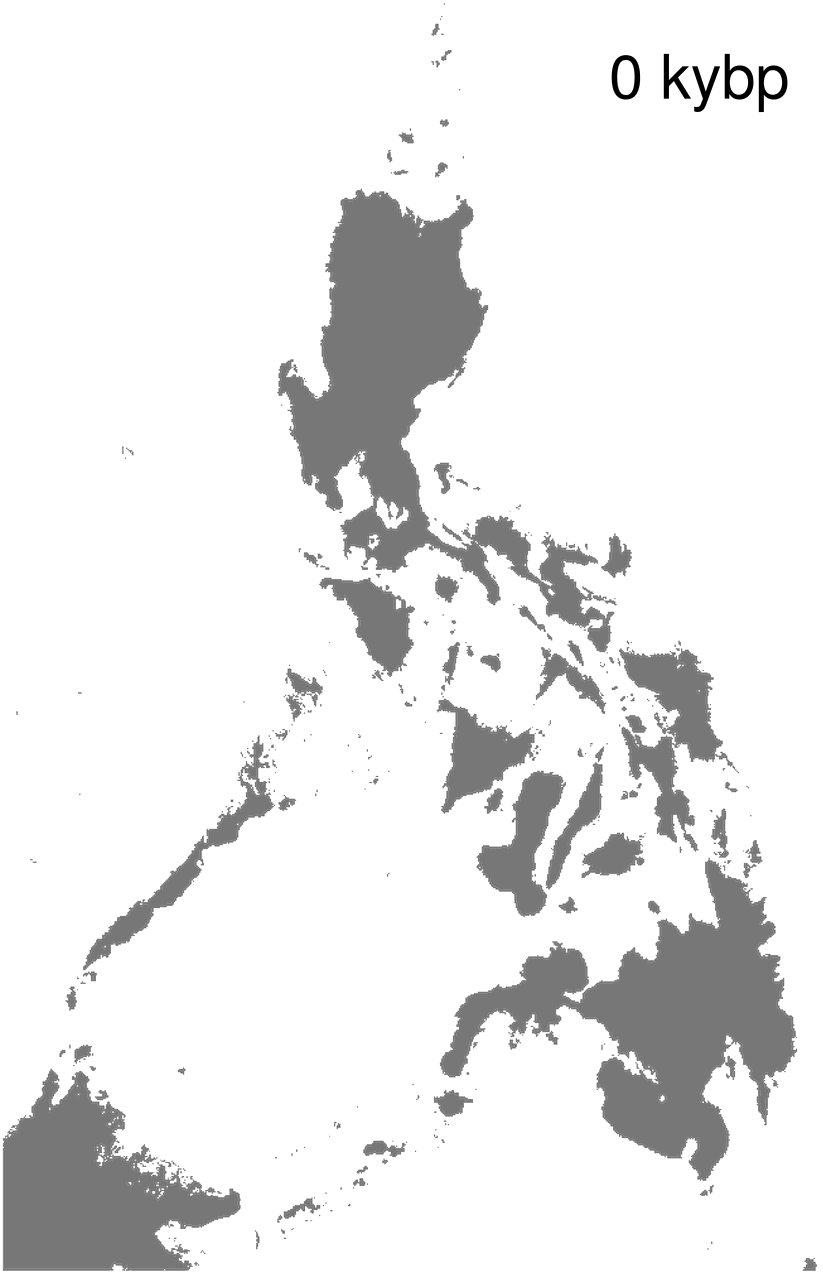
\includegraphics[height=0.8\textheight]{../../images/bathymetry-maps/animated-bathymetry-last-frame.png}}{VPlayer.swf}
    \captionsetup{name=Figure S, labelformat=noSpace, listformat=sFigList}
    \caption{
        \jroeditnoteb{New figure.}
        \jroeditb{}{%
        Animation of approximate sea-level changes in the Philippine Islands
        over the last 430,000 years.
        Sea-level estimates are from the projection of \citet{Spratt2016} based
        on seven reconstructions.
        Bathymetry data are from the ETOPO1 1-arc-minute global relief model
        \citep{Amante2009}.
        Animation generated using marmap version 1.0.2 \citep{Pante2013},
        ggplot2
        Version 2.2.1 \citep{ggplot2},
        \href{https://imagemagick.org/index.php}{ImageMagick}
        Version 6.9.10-8 Q16 x86\_64 20180723,
        and \href{https://ffmpeg.org/}{FFmpeg}
        Version 4.0.2-2.
        The source code for generating the plot is available at
        \url{https://github.com/phyletica/animating-sea-level-change}.
        This animation can also be viewed at
        \url{https://youtu.be/NjGdCezUvw8}.}
    }
    \label{fig:bathyanimation}
\end{center}
\end{figure}

\siFigure{../../../data/genomes/msg/ecoevolity-results/grid-cyrtodactylus-sumevents.pdf}{
    Approximate prior (light bars) and posterior (dark bars) probabilities
    of numbers of divergence events across pairs of \spp{Cyrtodactylus}
    populations
    under three different priors on the concentration parameter of
    the Dirichlet process.
    Bayes factors for each number of divergence times is given above the
    corresponding bars.
    Each Bayes factor compares the corresponding number of events 
    to all other possible numbers of divergence events.
    \weusedggplot
}{fig:cyrtneventsbyconcentration}

\siFigure{../../../data/genomes/msg/ecoevolity-results/grid-cyrtodactylus-sumtimes.pdf}{
    Approximate marginal posterior densities of divergence times for each
    pair of \spp{Cyrtodactylus} populations
    under three different priors on the concentration parameter of
    the Dirichlet process.
    \weusedggridges
}{fig:cyrtdivtimesbyconcentration}

\siFigure{../../../data/genomes/msg/ecoevolity-results/grid-cyrtodactylus-sumevents-nopoly.pdf}{
    Approximate prior (light bars) and posterior (dark bars) probabilities
    of numbers of divergence events across pairs of \spp{Cyrtodactylus}
    populations
    under four different combinations of prior on divergence times (rows)
    and recoding or removing polyallelic characters (columns).
    Bayes factors for each number of divergence times is given above the
    corresponding bars.
    Each Bayes factor compares the corresponding number of events 
    to all other possible numbers of divergence events.
    \weusedggplot
}{fig:cyrtneventsbytimeprior}

\siFigure{../../../data/genomes/msg/ecoevolity-results/grid-cyrtodactylus-sumtimes-nopoly.pdf}{
    Approximate marginal posterior densities of divergence times for each
    pair of \spp{Cyrtodactylus} populations
    under four different combinations of prior on divergence times (rows)
    and recoding or removing polyallelic characters (columns).
    \weusedggridges
}{fig:cyrtdivtimesbytimeprior}



\siFigure{../../../data/genomes/msg/ecoevolity-results/grid-cyrtodactylus-sumsizes.pdf}{
    Approximate marginal posterior densities of population sizes for each
    pair of \spp{Cyrtodactylus} populations
    under three different priors on the concentration parameter of
    the Dirichlet process.
    \weusedggridges
}{fig:cyrtpopsizesbyconcentration}

\siFigure{../../../data/genomes/msg/ecoevolity-results/grid-cyrtodactylus-sumsizes-nopoly.pdf}{
    Approximate marginal posterior densities of population sizes for each
    pair of \spp{Cyrtodactylus} populations
    under four different combinations of prior on divergence times (rows)
    and recoding or removing polyallelic characters (columns).
    \weusedggridges
}{fig:cyrtpopsizesbytimeprior}



\siFigure{../../../data/genomes/msg/ecoevolity-results/grid-gekko-sumevents.pdf}{
    Approximate prior (light bars) and posterior (dark bars) probabilities
    of numbers of divergence events across pairs of \spp{Gekko}
    populations
    under three different priors on the concentration parameter of
    the Dirichlet process.
    Bayes factors for each number of divergence times is given above the
    corresponding bars.
    Each Bayes factor compares the corresponding number of events 
    to all other possible numbers of divergence events.
    \weusedggplot
}{fig:gekkoneventsbyconcentration}

\siFigure{../../../data/genomes/msg/ecoevolity-results/grid-gekko-sumtimes.pdf}{
    Approximate marginal posterior densities of divergence times for each
    pair of \spp{Gekko} populations
    under three different priors on the concentration parameter of
    the Dirichlet process.
    \weusedggridges
}{fig:gekkodivtimesbyconcentration}

\siFigure{../../../data/genomes/msg/ecoevolity-results/grid-gekko-sumevents-nopoly.pdf}{
    Approximate prior (light bars) and posterior (dark bars) probabilities
    of numbers of divergence events across pairs of \spp{Gekko}
    populations
    under six different combinations of prior on divergence times (rows)
    and recoding or removing polyallelic characters (columns).
    Bayes factors for each number of divergence times is given above the
    corresponding bars.
    Each Bayes factor compares the corresponding number of events 
    to all other possible numbers of divergence events.
    \weusedggplot
}{fig:gekkoneventsbytimeprior}

\siFigure{../../../data/genomes/msg/ecoevolity-results/grid-gekko-sumtimes-nopoly.pdf}{
    Approximate marginal posterior densities of divergence times for each
    pair of \spp{Gekko} populations
    under six different combinations of prior on divergence times (rows)
    and recoding or removing polyallelic characters (columns).
    \weusedggridges
}{fig:gekkodivtimesbytimeprior}


\siFigure{../../../data/genomes/msg/ecoevolity-results/grid-gekko-sumsizes.pdf}{
    Approximate marginal posterior densities of population sizes for each
    pair of \spp{Gekko} populations
    under three different priors on the concentration parameter of
    the Dirichlet process.
    \weusedggridges
}{fig:gekkopopsizesbyconcentration}

\siFigure{../../../data/genomes/msg/ecoevolity-results/grid-gekko-sumsizes-nopoly.pdf}{
    Approximate marginal posterior densities of population sizes for each
    pair of \spp{Gekko} populations
    under six different combinations of prior on divergence times (rows)
    and recoding or removing polyallelic characters (columns).
    \weusedggridges
}{fig:gekkopopsizesbytimeprior}

\siFigure{../../../data/genomes/msg/ecoevolity-simulations/plots/ancestor-size-scatter.pdf}{
    \jroeditnote{New figure.}
    \jroedit{}{%
    The accuracy and precision of \ecoevolity estimates of the ancestral
    population size (scaled by the mutation rate) when applied to data
    simulated to match our \spp{Cyrtodactylus} (left) and \spp{Gekko} (right)
    RADseq \datasets with all sites (top) or only one SNP per locus (bottom).
    Each circle and associated error bars represent the posterior mean
    and 95\% credible interval.
    Estimates for which the potential-scale reduction factor
    % Details of the PSRF calculation are in the main text, so we
    % don't need this
    % \citep[PSRF; the square root of Equation 1.1 in][]{Brooks1998}
    was greater than 1.2
    \citep{Brooks1998} are highlighted in orange.
    Each plot consists of 4000 estimates---500 simulated \datasets, each with
    eight pairs of populations.
    For each plot, the root-mean-square error (RMSE) and the proportion of
    estimates for which the 95\% credible interval contained the true
    value---$p(\epopsize{}\murate{} \in \textrm{CI})$---is given.
    \weusedmatplotlib}
}{fig:simsancestralsizes}

\siFigure{../../../data/genomes/msg/ecoevolity-simulations/plots/descendant-size-scatter.pdf}{
    \jroeditnote{New figure.}
    \jroedit{}{%
    Accuracy and precision of \ecoevolity estimates of the descendant
    population sizes (scaled by the mutation rate) when applied to data
    simulated to match empirical \spp{Cyrtodactylus} (left) and \spp{Gekko} (right)
    RADseq \datasets with all sites (top) or only one SNP per locus (bottom).
    Each circle and associated error bars represents the posterior mean
    and 95\% credible interval.
    Estimates for which the potential-scale reduction factor
    % Details of the PSRF calculation are in the main text, so we
    % don't need this
    % \citep[PSRF; the square root of Equation 1.1 in][]{Brooks1998}
    was greater than 1.2
    \citep{Brooks1998} are highlighted in orange.
    Each plot consists of 8000 estimates---500 simulated \datasets, each with
    eight pairs of populations.
    For each plot, the root-mean-square error (RMSE) and the proportion of
    estimates for which the 95\% credible interval contained the true
    value---$p(\epopsize{}\murate{} \in \textrm{CI})$---is given.
    \weusedmatplotlib}
}{fig:simsdescendantsizes}

\siFigure{../../../data/genomes/msg/ecoevolity-simulations/plots/cyrt-event-time-sampling-disparity-scatter.pdf}{
    \jroeditnote{New figure.}
    \jroedit{}{%
    Accuracy and precision of \ecoevolity divergence-time estimates (in units
    of expected subsitutions per site) when applied to data simulated to match
    empirical RADseq \datasets sampled from the pairs of \spp{Cyrtodactylus
        philippinicus} populations from the islands of (left) Luzon and Babuyan
    Claro and (right) Polillo and Luzon
    (a subset of the results plotted in Figure~\ref{fig:simsdivtimes}).
    Results are shown for \ecoevolity analyses of \datasets that contain all
    sites (top), or only one SNP per locus (bottom).
    The number of individuals sampled from each island population is indicated
    in \jroeditb{parantheses}{parentheses} at the top of each column of plots.
    Results for these two pairs of populations are plotted separately here to
    compare divergence-times estimated from \datasets with large differences in
    the number of sampled individuals and loci.
    Each circle and associated error bars represents the posterior mean and 95\%
    credible interval for the time that a pair of populations diverged.
    Estimates for which the potential-scale reduction factor
    % Details of the PSRF calculation are in the main text, so we
    % don't need this
    % \citep[PSRF; the square root of Equation 1.1 in][]{Brooks1998}
    was greater than 1.2
    \citep{Brooks1998} are highlighted in orange.
    Each plot consists of 500 estimates---one from each of the 500 simulated
    \datasets.
    For each plot, the root-mean-square error (RMSE) and the proportion of
    estimates for which the 95\% credible interval contained the true
    value---$p(\comparisondivtime{} \in \textrm{CI})$---is given.
    \weusedmatplotlib}
}{fig:sampledisparitydivtimes}


\end{document}
